\documentclass[border=10pt]{standalone}
\usepackage{pgfplots}
\pgfplotsset{compat=1.9}

\begin{document}

% File: cyber_acp.jsonl.xlsx - Successfully Generated Policies: 109/120 (90.83%)
% File: t2p_acp.jsonl.xlsx - Successfully Generated Policies: 364/367 (99.18%)
% File: collected_acp.jsonl.xlsx - Successfully Generated Policies: 128/129 (99.22%)
% File: ibm_acp.jsonl.xlsx - Successfully Generated Policies: 119/129 (92.25%)
% File: acre_acp.jsonl.xlsx - Successfully Generated Policies: 482/499 (96.59%)
% File: xacml2_1.xml.xlsx - Successfully Generated Policies: 29/30 (96.67%)
% File: xacml2_2.xml.xlsx - Successfully Generated Policies: 27/30 (90.00%)
% File: xacml2_3.xml.xlsx - Successfully Generated Policies: 1466/1596 (91.85%)
% File: xacml3_1.xml.xlsx - Successfully Generated Policies: 2/2 (100.00%)
% File: xacml3_2.xml.xlsx - Successfully Generated Policies: 167/181 (92.27%)
% File: xacml3_3.xml.xlsx - Successfully Generated Policies: 12/12 (100.00%)

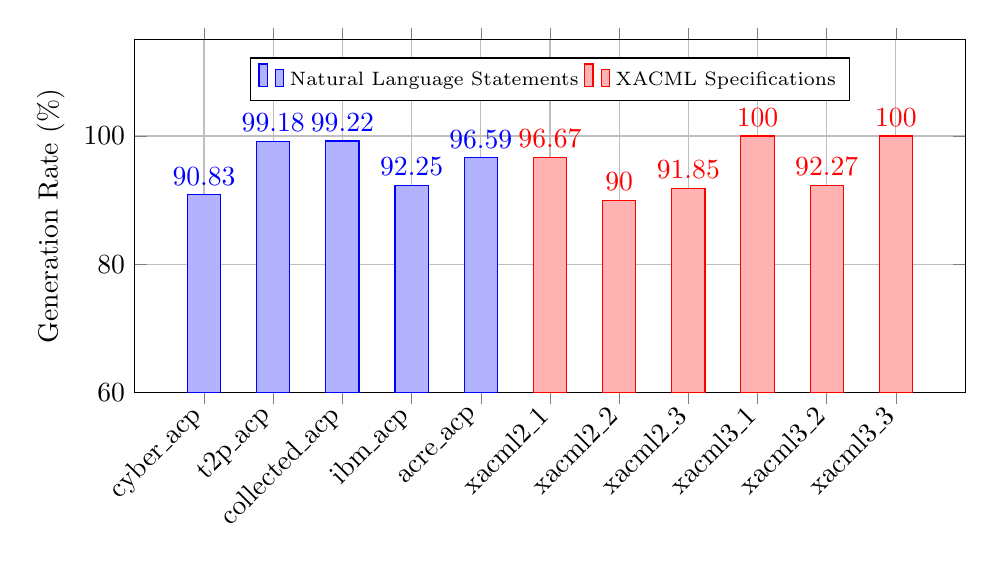
\begin{tikzpicture}
\begin{axis}[
    ybar,
    bar width=12pt,
    width=\textwidth,
    height=0.5\textwidth,
    ymin=60,
    ymax=115,
    ylabel={Generation Rate (\%)},
    symbolic x coords={cyber\_acp, t2p\_acp, collected\_acp, ibm\_acp, acre\_acp, xacml2\_1, xacml2\_2, xacml2\_3, xacml3\_1, xacml3\_2, xacml3\_3},
    xtick={cyber\_acp, t2p\_acp, collected\_acp, ibm\_acp, acre\_acp, xacml2\_1, xacml2\_2, xacml2\_3, xacml3\_1, xacml3\_2, xacml3\_3},
    x tick label style={rotate=45, anchor=east},        
    nodes near coords,
    enlarge x limits=0.1,
    grid=major,
    legend style={legend columns=2, font=\scriptsize, at={(0.5,0.95)}, anchor=north},
    ]
\addplot+[bar shift=0pt] coordinates {
    (cyber\_acp, 90.83)
    (t2p\_acp, 99.18)
    (collected\_acp, 99.22)
    (ibm\_acp, 92.25)
    (acre\_acp, 96.59)
};
\addplot+[bar shift=0pt] coordinates {
    (xacml2\_1, 96.67)
    (xacml2\_2, 90.00)
    (xacml2\_3, 91.85)
    (xacml3\_1, 100.00)
    (xacml3\_2, 92.27)
    (xacml3\_3, 100.00)
};
\legend{Natural Language Statements, XACML Specifications}
\end{axis}
\end{tikzpicture}

\end{document}
